
% titlepage-demo.tex
\documentclass{beamer}
\usetheme{Boadilla}
\usepackage{multirow}
\usepackage[absolute,overlay]{textpos} 
\newenvironment{reference}[2]{% 
  \begin{textblock*}{\textwidth}(#1,#2) 
      \footnotesize\it\bgroup\color{red!50!black}}{\egroup\end{textblock*}} 

\begin{document}

\begin{frame}[t]{Next Study}
\begin{center}
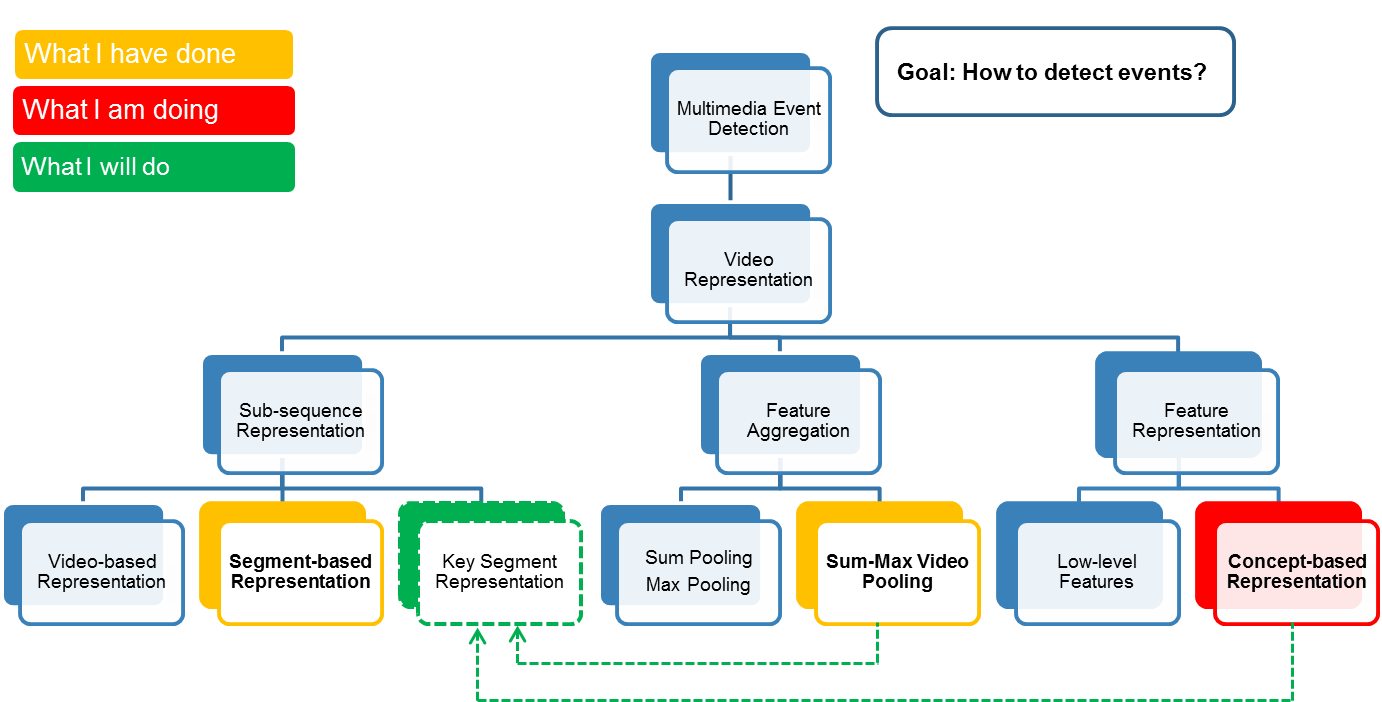
\includegraphics[width=12cm,height=7cm]{images/bigpicture2.png}
\end{center}

\end{frame}

\begin{frame}[t]{Toward Key Segment Selection for MED}

\begin{definition}
Key segments: segments that contain positive evidence for a specific event
\end{definition}

\begin{itemize}
\item Existing work addresses the problem without identification of key segments. 
\item Video level features are aggregated over the entire videos.
\end{itemize}

\textbf{Drawback}: Each part of the video contributes equally to the final representation $\rightarrow$ making it prone to noise. 

\textbf{For our segment-based approach}: features are aggregated over the uniform sampled segments $\rightarrow$ might not contain key segments

\textbf{Research Problem}: How about automatically finding the key segments that contain positive evidence for a specific event?

\end{frame}

\begin{frame}[t]{Toward Key Segment Selection for MED}
	Mapping the results of visual processing and text processing into a common space.
	\begin{center}
		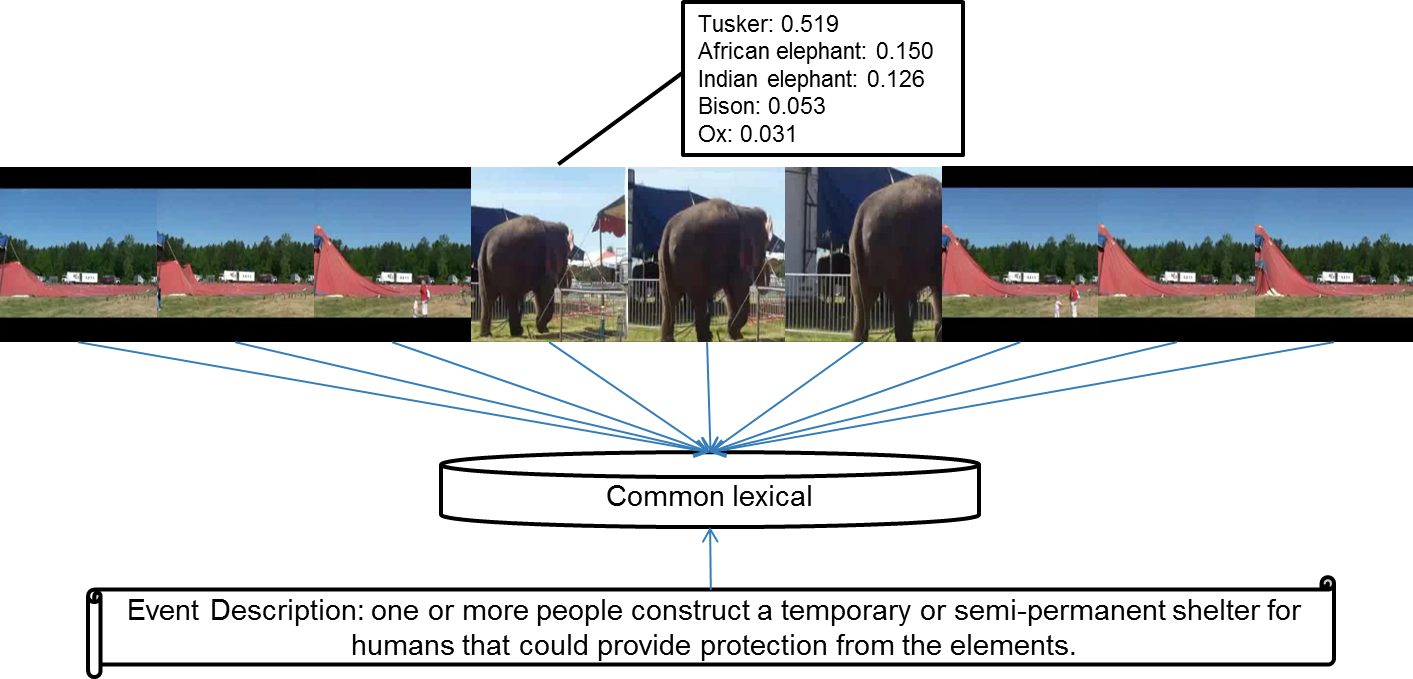
\includegraphics[width=12cm,height=7cm]{images2/toward1.png}
	\end{center}
\end{frame}

\begin{frame}[t]{Toward Key Segment Selection for MED}
	\begin{itemize}
		\item Merging keyframe similarity to calculate segment similarity. 
		\item Key segments are segments that have high similarity to the event description.
	\end{itemize}

	\begin{center}
		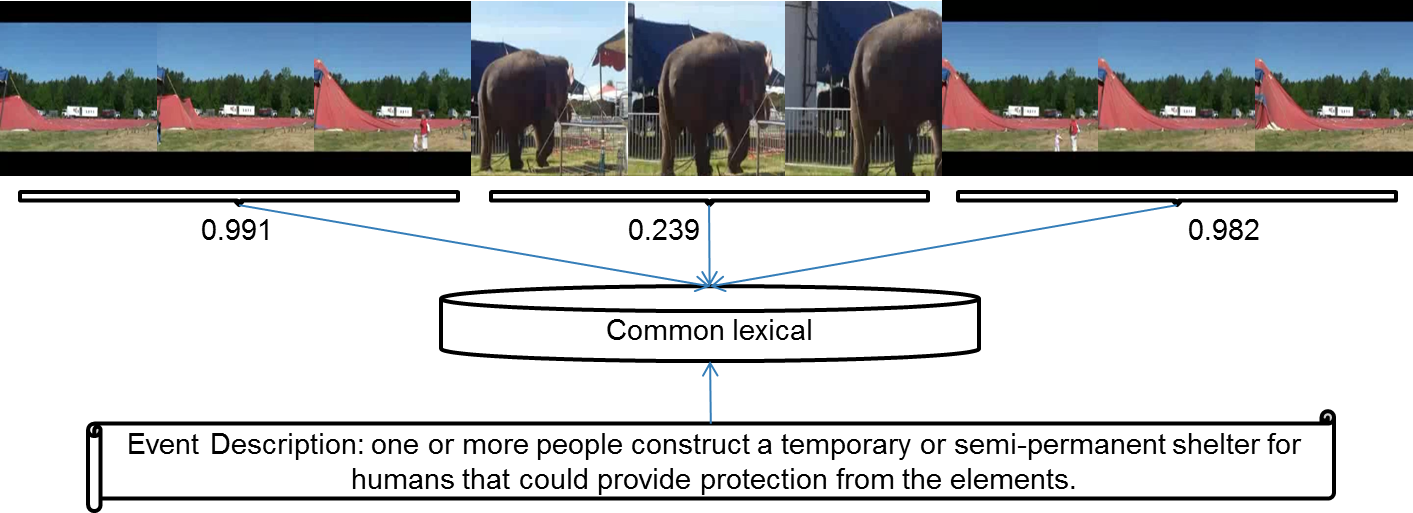
\includegraphics[width=12cm,height=6cm]{images2/toward2.png}
	\end{center}
\end{frame}
	
\begin{frame}[t]{Then...}
\begin{itemize}
\item Apply Sum-max Video Pooling.
\item Extend to Weighted Sum-max Video Pooling.
\item How to impose temporal relationship between segments?

\begin{itemize}
\item Assembling a shelter: people should gathering before assembling
\begin{center}
	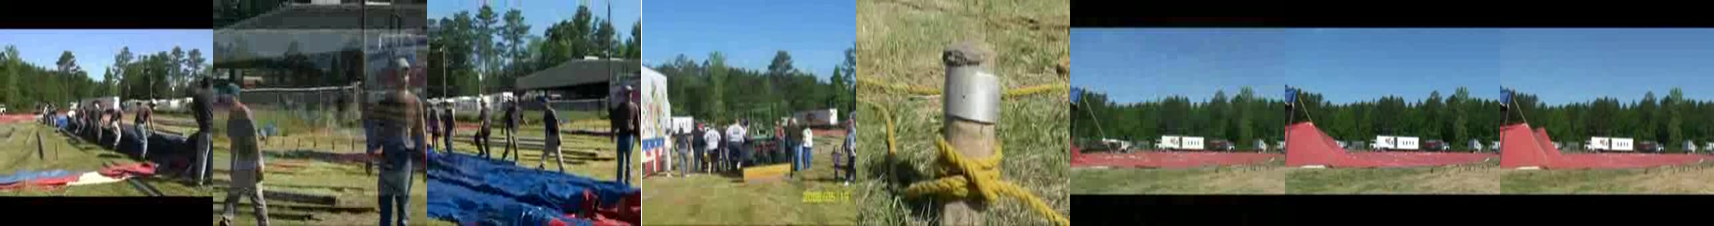
\includegraphics[width=10cm,height=2.5cm]{images2/temporal.png}
\end{center}
\item Birthday party: people often singing before blowing candle and then eating
\end{itemize}
$\rightarrow$ Language knowledge might help to incorporate these constraints.	
\end{itemize}
\end{frame}

\begin{frame}[t]{Automatic Video2Text Generation}
	[collaboration work with Prof. Yusuke Miyao, NII]
	\begin{itemize}
		\item We aim to generate text descriptions for key segments, as well as the whole video.
\begin{center}
	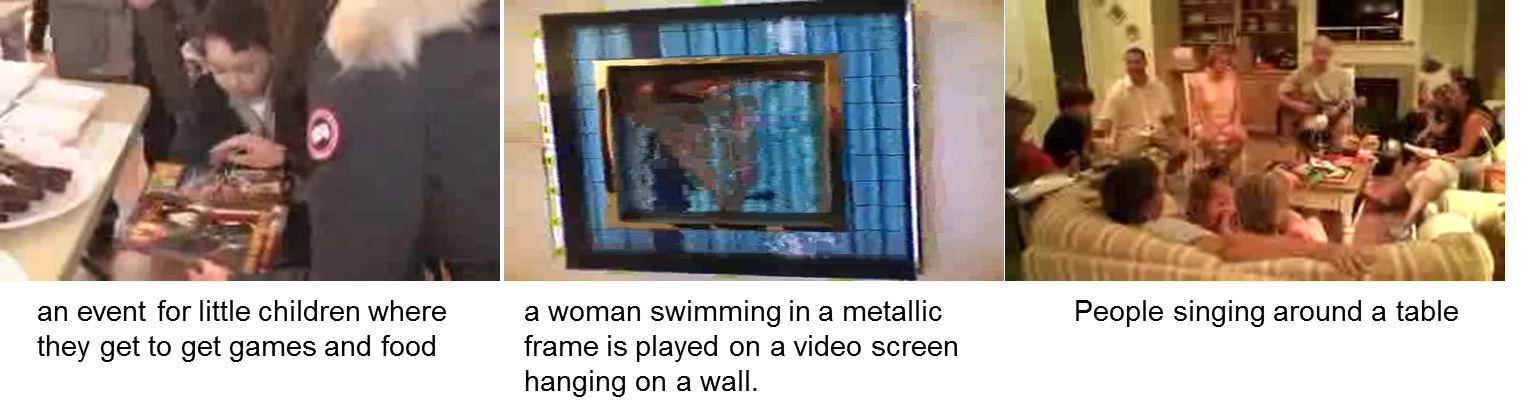
\includegraphics[width=10cm,height=3cm]{images2/nlpproject.png}
\end{center}
	\item The results of this project can be used for event recounting, i.e. provide evidences for event detection.
	\item We are building a VideoNet for action classification in real world situation.		
	\end{itemize}
\end{frame}
	
\end{document}